\documentclass[]{article}
\usepackage{graphicx}
\usepackage{geometry}
%\usepackage{showframe} %This line can be used to clearly show the new margins

\newgeometry{vmargin={15mm}, hmargin={15mm,20mm}}   % set the margins

% Title Page
\title{The Battleship Game}
\author{Pavel Mačák}


\begin{document}
\maketitle

\section{Intoduciton}

Welcome to The Battleship Game. It is World War Two and you are a fresh gunner recruit in the Royal Navy. Together with yout friend you still haven't experienced the true horrors of war. Even better, the spotter on your deck is too unskilled (and mostly drunk) to report position of enemy ships properly. He only reports when you hit something, but for the rest you are practically shooting blind. That is why you make each battle a bit more fun for yourself.

You take turns shooting the big 120mm gun, keeping track of the hits you make. The enemy armada has different ships at their disposal. Damaging or even sinking the enemy capital ships is of course a much bigger success than just putting some screens (such as destroyers) out of business. So you made up a scoring system. For each type of ship, there different points are awarded. You get double of it for sinking a ship completely. Sometimes your friend (the second player) can be a crybaby, so if you feel like it, you can give him a tiny advantage, by counting your hits for less points.


\begin{figure}
	\centering
	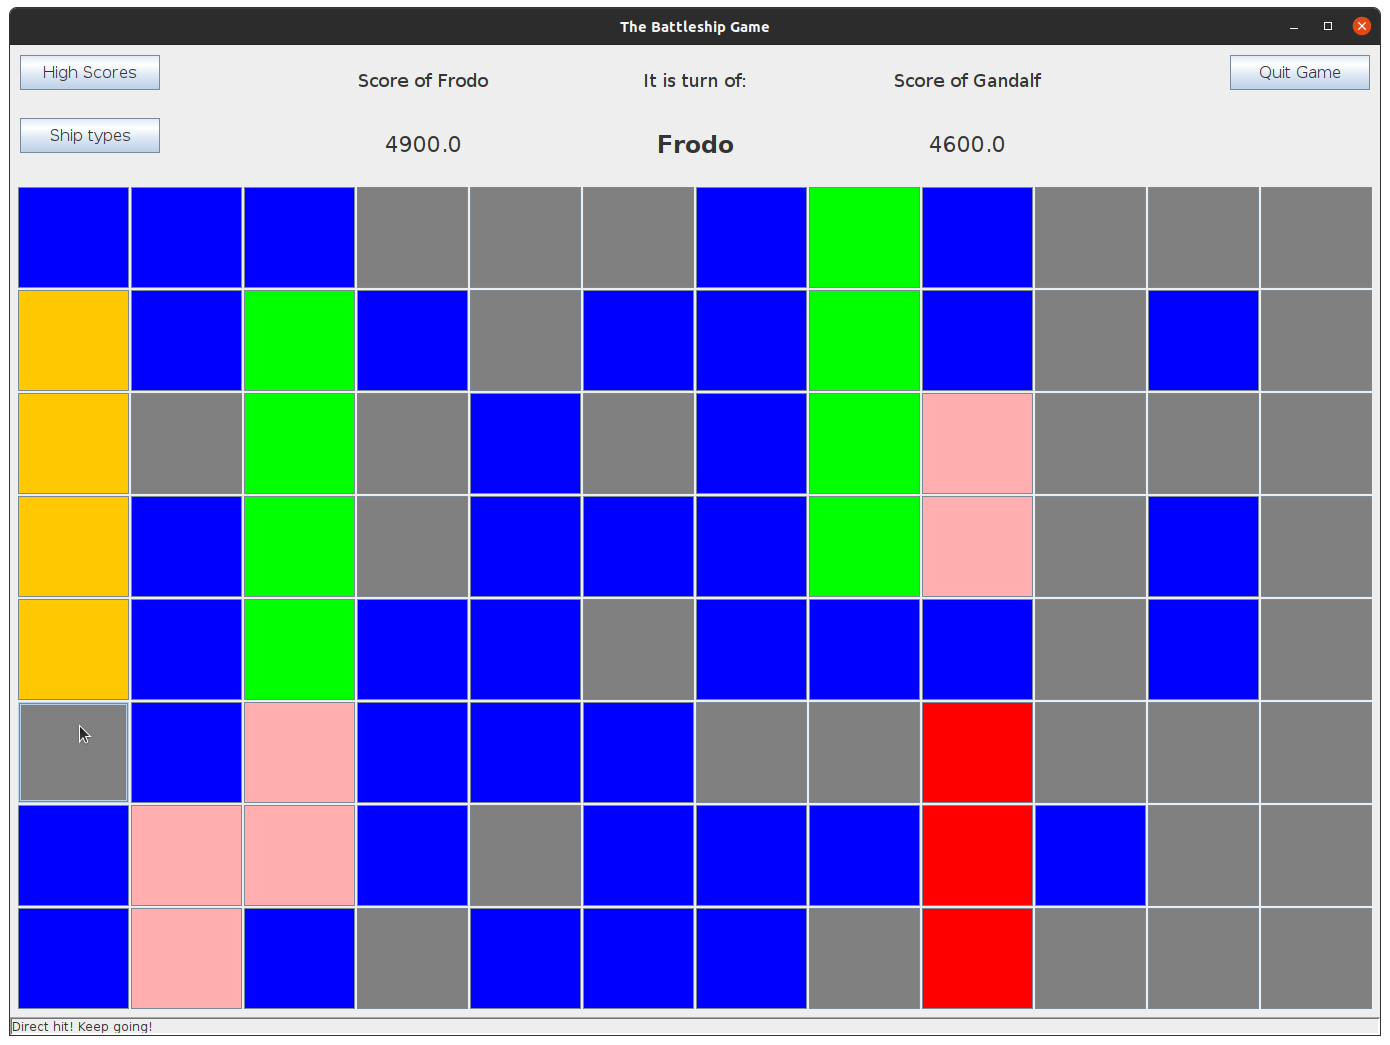
\includegraphics[width=0.7\linewidth]{figs/boardScreen}
	\caption{This is how the board can look like before the game ends.}
	\label{fig:boardscreen}
\end{figure}

\section{Rules and how-to}
The two players take turns in shooting at enemy ships. You do this by clicking on any of the gray tiles, which represent places that have not been hit yet. When a player hits a ship, he may fire again, but if that hit results in the ship sinking, the turn goes to the other player. The game will end once the enemy fleet is completely destroyed.
\begin{itemize}
	\item When a player hits a ship he is awarded points acording to the type of ship he/she hit.
	\item Sinking a ship (hitting its last tile) awards double the points for only hitting the ship.
\end{itemize}

When the application starts, you will see the main menu screen (Figure \ref{fig:menuscreenshot}). Here you can set the names of both players, look at recap of the rules, see the high scores or tweak your gaming experience. The two buttons above the players' names serve this purpose. Firstly, you can change the scoring system giving the starting player some disadvantage. Secondly, you can change the size of the board and the placement of the ships as well as their numbers (although be careful when putting too many ships). The placement can be done at random or using a file with this format:

\begin{verbatim}
	8 12
	Carrier;3*2;3*3;3*4;3*5;3*6
	Battleship;5*6;6*6;7*6;8*6
	Submarine;5*2;6*2;7*2;
	Destroyer;1*7;1*8
\end{verbatim}
The two numbers on first line specify the board sizes. If there is only one number, the board will be a square. The name of the ship type and coordinates are each separated from one another by a semicolon. A coordinate is specified by two numbers separated by a “*” with the first number representing the row and the second number representing the column. For example, “2*3” represents the tile at row 2 and column 3 of the board.

\begin{figure}[h]
	\centering
	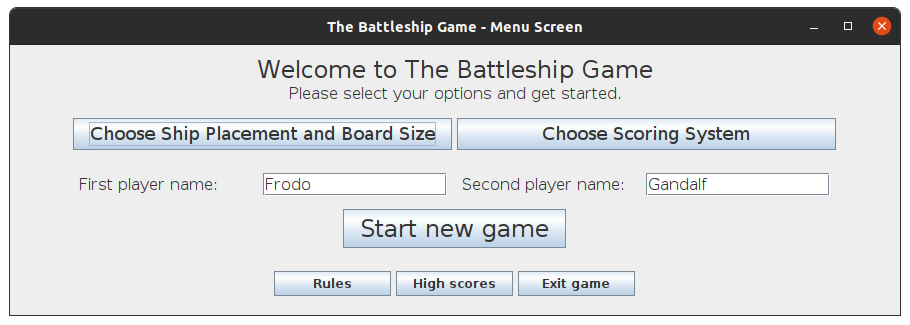
\includegraphics[width=0.7\linewidth]{figs/menuScreenshot}
	\caption{Main menu screen.}
	\label{fig:menuscreenshot}
\end{figure}

If you want to play more games be sure to generate/load a new board each time, otherwise it will stay the same.
\newpage

\section{Code description}

\subsection{Classes}
\subsubsection{Application package}
\begin{itemize}
	\itemsep0em 
	\item \texttt{BoardSetup} Class holding necessary variables to initialize an instance of Board.
	\item \texttt{HighScore} Class holding a single high score and name of the player who scored it.
	\item \texttt{HighScoreManager} Class managing high scores, loading and saving them to a file.
	\item \texttt{InputFileLine} Helper class for reading ship placements from file.
	\item \texttt{ShipCounter} Class keeping track of how many ships should be put on board when generating random placements.
\end{itemize}

\subsubsection{Implementation package}
\begin{itemize}
	\itemsep0em 
	\item \texttt{Board} Class representing board that the game is played on.
	\item \texttt{Coords} Simple class holding two integer coordinates. Class name is abbreviation for Coordinates.
	\item \texttt{Game} Instance of this class represents a game that is played.
	\item \texttt{HitType} Enum of type of hits a player can make - miss, hit and sink.
	\item \texttt{Placement}Abstract class. Represents placement on tile grid. Concrete examples could be Linear, Square, Cross placements.
	\subitem \texttt{LinearPlacement} Class holding placement of objects on the Board. Allow only for linear placement, meaning it will throw exceptions if constructed to be anything else apart from one cell or a column or row of cells. Implements the Iterable interface to iterate through list of coordinates.
	\item \texttt{Player} Class representing a player playing the game.
	\item \texttt{ScoringSystem} Abstract interface for different scoring systems.
	\subitem \texttt{EqualScoringSystem} Both Players get the same amount of points.
	\subitem \texttt{UnequalScoringSystem} Players get different amount of points.
	\subsubitem \texttt{HandicapScoringSystem} Player gets a multiplier on his scores.
	\subsubitem \texttt{SubstractScoringSystem} Player gets a value substracted from his scores.
	\item \texttt{Ship} A class representing a ship.
	\item \texttt{ShipList} Class holding a list of ships.
	\item \texttt{ShipType} Enum holding types of ships. New types of ships can be added here.
	\item \texttt{Tile} Abstract class. Represents a tile on the Board.
	\subitem \texttt{ShipTile} Class representing a tile with a ship on it.
	\subitem \texttt{WaterTile} Class representing an empty tile on the board.
	\item \texttt{TileColor} Enum of colors that a tile can have. This was created before starting with the GUI to make it easier later.
\end{itemize}

\subsection{GUI package}

\begin{itemize}
	\itemsep0em 
	\item \texttt{Control} Main class controlling the flow of the program.
	\item \texttt{GameFrame} JFrame extension - a window for actually playing the game.
	\item \texttt{HighScoreDialog} \texttt{showDialog} method that displays the high scores.
	\item \texttt{MainFrame} The main menu window.
	\item \texttt{MyUtils} Some funtions to save time writing the same code.
	\item \texttt{PlacementDialog} Dialog window for setting ship placement and ship numbers.
	\item \texttt{ScoringSystemDialog} Dialog for choosing the scoring system.
	\item \texttt{Texts} Enum with some texts. There is probably a smarter way to save long foramted texts in Java, but I haven't looked for it at the moment.
\end{itemize}

\subsection{Relationships}
To start with the main game logic, the class \texttt{Game} is of main interest. It receives inputs in terms of function \texttt{clickOnTile} which processes a mouse click (for GUI application) or a console input (for a text application). It makes use of the class \texttt{Player} to represent the two players, the general \texttt{ScoringSystem} interface to distinguish between different scoring systems and the \texttt{Board} class which basically holds the information on the tiles as well as exposing some methods to manipulate them. The \texttt{Tile} class itself is abstract base class for the implementations \texttt{ShipTile} and \texttt{WaterTile}. Coming back a bit, the \texttt{Board} class also holds the list of ships (the custom \texttt{ShipList} class) that are placed on the board. The \texttt{Ship} objects in this list are also assigned to corresponding tiles and keep track of the Ship status. Each ship is of one type which are defined in \texttt{ShipType} enumerator. The \texttt{ScoringSystem} interface has one method which takes the normal points that should be scored and a player that should score and recalculates the points if necessary.

The application package has classes which deal with file I/O - mainly the \texttt{BoardSetup} which exposes methods of initializing \texttt{ShipList} from file or randomly. It is then used in the constructor of \texttt{Board} when a new game is started. High scores saving and loading is handled by \texttt{HighScoreManager} which makes use of \texttt{HighScore} class to hold information about a high score entry. An instance of \texttt{ShipCounter} is passed to \texttt{BoardSetup} when initializing the ship list at random and is also used by the GUI so that the user may chose the ship numbers.

The visualization package implements GUI elements. The \texttt{MainFrame} is the main menu window which subsequently calls settings dialogs -\texttt{Placement} and \texttt{ScoringSystem} as well as information dialogs with rules and high scores (\texttt{HighScoresDialog}, also used by \texttt{GameFrame}). It extends the \texttt{JFrame} class because it overrires the \texttt{dispose()} method to always ask user for confirmation before exiting the program. It also hold game logic elements for scoring systems, board setup and high score manager. The game window is implemented in \texttt{GameFrame} class and basically takes an instance of \texttt{Game} that the user wants to play and gets all the necessary information out of that object.


\section{Strengths, weaknesses and difficulties}

The main game logic is designed to be general. Some more ship types can be easily added in the \texttt{ShipType} enum and the game will work with them. It should also be quite easy to implement new game objects such as islands or naval bases of different shapes (now it is only line or a single tile). Only the implementation of scoring systems is a bit less general - the double for sinking rule is actually hard coded. Possible solution could be passing the \texttt{HitType} (and maybe even \texttt{ShipType}) to scoring systems as well so the decision can be made there.

The GUI code is pretty ugly, but it took me much more time than I expected to get it working at least like this, but with this experience i would do organize it a bit differently. On the other hand i think I did a pretty good job in keeping game logic and the GUI separated. 

difficulties when running multiple games in one program instance (i.e. without restarting the program) because I actually didn't have that in mind when designing the application (which was a mistake). To make this work I had to use some hard copying (of \texttt{ShipList} when creating an instance of \texttt{Board}) which is not the cleanest way to do it I suppose.

As was suggested by someone on the Discussion board, the player keeps their turn if they hit a ship. This made more sense to me in terms of gameplay, while not needing extra time to make it work.

Also customizing ship numbers is a quite good feature in mine opinion because than it makes sense to increase the board size as well. For me it was also a bit more natural to allow any number of ships than hard coding that each ship is may be placed only once.

Further optimizations regarding code readability could still be done by avoiding boilerplate code using lombok annotation for data classes, assignment constructors etc.

\end{document}          
